% !TEX root = onlinevarinancebandits.tex


\section{The Bandit Setting} \label{sec:bandit}
In this section, we investigate the bandit setting (see Figure~\ref{fig:Protocal_bandit}) which is of great practical appeal as we described in Section~\ref{sec:Motivation}.
Our method for the bandit setting is depicted in Algorithm~\ref{alg:bandit}, and it ensures a bound of $\tilde{O}(n^{1/3}T^{2/3})$ on the expected  regret (see Theorem~\ref{thm:bandit-non-oblivious}). Importantly, this bound holds even for non-oblivious adversaries.
The design and analysis of our method builds on some of the ideas that appeared in the  seminal work of  \cite{auer2002nonstochastic}. 

Algorithm~\ref{alg:bandit} is using the bandit feedback in order to design an unbiased estimate of the true loss  $(\ell_t(1),\ldots,\ell_t(n))$ in each round. These estimates are then used instead of the true losses by the full information FTRL algorithm that was analyzed in the previous section.  We do not directly play according to the FTRL predictions but rather mix them with a uniform distribution. Mixing is necessary in order to ensure that the   loss estimates are bounded, which is  a crucial  condition used in the analysis. Next we elaborate  on our method and its analysis.
%Inspired by the EXP3 algorithm which is designed to solve the bandit setting with linear costs, we design a
%
%
%In order to address some of the challenges in this setting we adopt some of the ideas that are used in the EXP3 which 
%
%The full information setting is unrealistic for practical applications, since we assume that we observe the feedback for all arms in each round. This setup only serves as a mean for extension to the bandit setting, which we investigate in this section where we use tools from the design of the EXP3 algorithm. 

Algorithm~\ref{alg:bandit} samples an arm $I_t\sim \tp_t$ at every round, and receives a bandit feedback $\ell_t(I_t)$. 
This may be used in order to construct an estimate of the true (squared) loss as follows,
%
%
%Inspired by [Auer et al]
%A simple idea to compensate for observing only the feedback for one chose arm $I_t$  is to employ an unbiased estimate of the squared loss function
\begin{equation*}
\tell_t^2(i) := \frac{\ell_t^2(i)}{\tp_t(i)}\cdot \mathbbm{1} _{I_t=i}~,
\end{equation*}
and it is immediate to validate that the above is unbiased in the following sense, 
\begin{equation*}
\mathbb{E}[\tell_t^2(i) \vert \tp_t,\ell_t] = \ell_t^2(i),\quad \forall i\in[n].
\end{equation*}
Analogously to the previous section it is natural to define modified cost functions as 
\begin{equation*}
\tf_t(p) = \sumin {\tell_t^2(i)}/{p(i)}~.
\end{equation*}
Clearly, $\tf_t$ is an unbiased estimate of the true cost, $\mathbb{E}[\tf_t(p) \vert \tp_t,\ell_t] = f_t(p)$.
From now on  we omit the conditioning on $\tp_t,\ell_t$ for notational brevity. 
%and define $\tf_t(p) = \sumin \frac{\tell_t^2(i)}{p(i)}$ analogously to the previous section
%In the following analysis we omit the conditioning on $p_t,\ell_t$ for notational brevity. 
Having devised an unbiased estimate, we could return to the full information analysis of FTRL with the modified losses. However, this poses a difficulty, since the modified losses  can possibly be unbounded. We remedy this by mixing the FTRL output, $p_t$, with a uniform distribution.
Mixing encourages exploration, and in turn gives a handle on the possibly unbounded modified losses. Let $\theta\in [0,1]$, and define,
\begin{equation*}
\tp_t(i) = (1-\theta)\cdot p_t(i) +{\theta}/{n}.
\end{equation*}
Since $\tp_t(i) \geq \theta / n$, we have $\tell_t^2(i) \leq nL/\theta$. We summarize the resulting method\footnote{The
sampling and update in the presented form have a complexity of $\mathcal{O}(n)$. 
%which renders the method impractical. 
There is a standard way to improve this issue based on segment trees that gives $\mathcal{O}(\log n)$ for sampling and update. A detailed description of this idea can be found in section A.4. of \cite{salehi2017stochastic}} in Figure \ref{alg:bandit}.
%   \begin{algorithm}[t]
%             \caption{Variance Reducer Bandit}
%             \label{alg:bandit}
%             \begin{algorithmic}
%      \State {\bfseries Input:} $\theta$, $L$, $n$
%      \State Initialize $w(i)=0$ for all $i \in [n].$
%      \For{$t=1$ {\bfseries to}  $T$}
%        \State $p_t(i) \propto \sqrt{w(i) + L\cdot n / \theta}$
%       \State $\tp_t(i) = (1-\theta) \cdot p_t(i) + {\theta}/{n}$,  for all $i \in [n]$
%         \State Draw $I_t \sim \tp_t$ and play $I_t$.
%         \State Receive feedback $l_t(I_t)$, and update $w(I_t) \gets w(I_t) + l^2_t(I_t) / \tp_t(I_t)$.
%         %\State $w(I_t) = w(I_t) + l^2_t(I_t) / \tp_t(I_t)$
%      \EndFor
%   \end{algorithmic}
%      \end{algorithm}
\begin{figure}[t]
\begin{framed}
\centering{ \textbf{Variance Reducer Bandit (VRB)}\\}
 \flushleft
 \textbf{Input}: $\theta$, $L$, $n$ \\
 Initialize $w(i)=0$ for all $i \in [n].$\\
   \textbf{for} $t=1,\ldots, T$ \textbf{do} \\
   \quad{ $p_t(i) \propto \sqrt{w(i) + L\cdot n / \theta}$\\
   \quad{ $\tp_t(i) = (1-\theta) \cdot p_t(i) + {\theta}/{n}$,  for all $i \in [n]$} \\
   \quad{ Draw $I_t \sim \tp_t$ and play $I_t$.} }\\
   \quad{ Receive feedback $l_t(I_t)$, and update $w(I_t) \gets w(I_t) + l^2_t(I_t) / \tp_t(I_t)$.} \\
      \textbf{end for} \\
\end{framed}
\caption{Variance Reducer Bandit}
\label{alg:bandit}
\end{figure}
     
     
We start with analyzing the \emph{pseudo-regret} of our algorithm, where we compare the cost incurred by the algorithm to the cost incurred by the optimal distribution \emph{in expectation}. The pseudo-regret is defined below,
\begin{equation} \label{eq:bandit-regret}
\frac{1}{n^2}\min_{p \in \Delta }  \expval{   \sumtt f_t(\tp_t)  -  \sumtt f_t(p)},
\end{equation}
where the expectation is taken with respect to both the player's choices and the loss realizations. The pseudo-regret is only a lower bound for the \emph{expected regret}, with  an equality when the adversary is oblivious, i.e., does not take the past choices of the player into account.

\begin{theorem} \label{thm:bandit-main}
Let $\theta = (n/T)^{1/3}$.
Assuming $T \geq n$, the algorithm in Figure~\ref{alg:bandit} ensures the following bound:
% the following holds for the pseudo-regret
\begin{equation*}
\frac{1}{n^2}\min_{p \in \Delta }  \expval{   \sumtt f_t(\tp_t)  -  \sumtt f_t(p)} \leq 74Ln^{\frac{1}{3}}T^{\frac{2}{3}}.
\end{equation*}
\end{theorem}

\begin{proofarg}{sketch of Theorem~\ref{thm:bandit-main}}
%Due to the law of total expectation we have
Using the unbiasedness of the modified costs we have
\begin{equation*}
 \min_{p \in \Delta } \expval{   \sumtt f_t(\tp_t)  - \sumtt f_t(p)} 
= \min_{p \in \Delta }  \expval{   \sumtt \tf_t(\tp_t)  -  \sumtt \tf_t(p)} .
\end{equation*}
We can decompose $\frac{1}{n^2} \min_{p \in \Delta } \expval{   \sumtt \tf_t(\tp_t)  -  \sumtt \tf_t(p)} $  into the following terms:
\begin{align*}
&\uann{ \frac{1}{n^2}\expval {\sumtt \tf_t(\tp_t) - \sumtt \tf_t(p_t)  } } {\rA} + \uann{\frac{1}{n^2} \min_{p \in \Delta } \expval{\sumtt \tf_t(p_t)  - \sumtt \tf_t(p)   } }{\rB}
\end{align*}
where $\rA$ is the cost we incur by mixing, and $\rB$ is upper bounded by the regret of playing FTRL with the modified losses. Now we inspect each term separately. 

An upper bound of $  \theta  L  T$ on $\rA$ results from the  simple observation that 
$
1/\tp_t(i)- 1/p_t(i) \leq n \theta.
$
For bounding $\rB$, notice that  $p_t$ is   performing FTRL over the modified cost sequence. Combining this together the  bound $\tell_t^2(i) \leq nL/\theta$ allows us to apply Theorem \ref{thm:full-info-main} and get,
%we can reuse the result in Theorem \ref{thm:full-info-main} with the modified losses:
\begin{equation}\label{eq:RegretModifiedCosts}
\frac{1}{n^2}\left( \sumtt \tf_t(p_t)  - \min_{p \in \Delta } \sumtt \tf_t(p) \right)
 \leq 
  27 \sqrt{\frac{L}{n \theta}}\left(\sum_{i=1}^n \sqrt{ \tell_{1:T}^2(i) }  \right) +\frac{44nL}{\theta} ~.
\end{equation}
Due to Jensen's inequality we have 
$
\expval{\sum_{i=1}^n  \sqrt{\tell_{1:T}^2(i)}} 
%= \sum_{i=1}^n \expval{ \sqrt{\tell_{1:T}^2(i)}}
 \leq \sum_{i=1}^n \sqrt{\expval{\tell_{1:T}^2(i)}} = \sum_{i=1}^n \sqrt{\ell_{1:T}^2(i)} 
$.
Finally, we get an upper bound on the pseudo-regret which we can optimize in terms of $\theta$:
\begin{equation*}
\frac{1}{n^2}  \min_{p \in \Delta }  \expval{   \sumtt f_t(\tp_t)  -  \sumtt f_t(p)} \leq \theta LT +27\sqrt{\frac{L}{n \theta}}\left(\sum_{i=1}^n \sqrt{ \ell_{1:T}^2(i) }  \right) +\frac{44nL}{\theta} .
\end{equation*}
Using the bound $\sum_{i=1}^n \sqrt{ \ell_{1:T}^2(i) }\leq n \sqrt{LT}$ and the assumption $T\geq n$, we set $\theta = (n/T)^{1/3}$ to get the result. Note that  $\theta$ is dependent on knowing $T$ in advance. If we do not assume that this is possible, we can use the ``doubling trick'' starting from $T=n$, and incur an additional constant multiplier in the regret.
\end{proofarg}

Ultimately, we are interested in the \emph{expected regret}, where the adversary is allowed to make decisions by taking into account the player's past choices, i.e., to be \emph{non-oblivious}. 
We present the main result of this paper, which establishes a $\tO(n^{1/3}T^{2/3})$  regret bound, where the $\tO$ notation hides the logarithmic factors.

\begin{theorem} \label{thm:bandit-non-oblivious}
Assuming $T \geq n$, the following holds for the expected regret:
\begin{equation*}
\frac{1}{n^2} \expval{   \sumtt f_t(\tp_t)  - \min_{p \in \Delta }  \sumtt f_t(p)} \leq \tilde{\mathcal{O}}\left(Ln^{\frac{1}{3}}T^{\frac{2}{3}}\right).
\end{equation*}
\end{theorem}

\begin{proofarg}{sketch of Theorem~\ref{thm:bandit-non-oblivious}}
Using the unbiasedness of the modified costs allows to decompose the regret as follows,
\begin{align} \label{eq:MasterNonOblivious} 
n^2\expval{ \regret_T } 
&=  
\expval{   \sumtt \tf_t(\tp_t)  - \min_{p \in \Delta }  \sumtt \tf_t(p)}
+\expval{  \min_{p \in \Delta }  \sumtt \tf_t(p)  - \min_{p \in \Delta }  \sumtt f_t(p)}  \nonumber\\
&\leq
n^2\mathcal{O}(Ln^{1/3}T^{2/3}) 
+ 
\expval{  
\underset{\rA}{ \underbrace{
 \left(\sumin \sqrt{\tell_{1:T}^2(i)}  \right)^2 -  \left(\sumin \sqrt{\ell_{1:T}^2(i)}  \right)^2
 }}
 },
\end{align}
where  the last line uses  Equation~\eqref{eq:RegretModifiedCosts}  together with  Jensen's inequality (similarly to the proof of Theorem~\ref{thm:bandit-main}). We have also used the closed form solution for the minimal values of  $\sum_t f_t(p)$ and $\sum_t \tf_t(p)$ over the simplex. 

Our approach  to bounding  the remaining term is to establish  high probability bound for $\rA$. In order to do so we shall bound the following differences $\tell_{1:T}^2(i) - \ell_{1:T}^2(i)$. This can be done by applying the 
\vspace{10pt}
appropriate concentration results described below. \\
\textbf{Bounding  $\tell_{1:T}^2(i) - \ell_{1:T}^2(i)$.}
Fix $i\in[n]$ and define $Z_{t,i}:=\tell_t^2(i) - \ell_t^2(i)$. Recalling that \linebreak $\mathbb{E}[\tell_t^2(i) \vert \tp_t,\ell_t] = \ell_t^2(i)$, we have that $\{ Z_{t,i}\}_{t\in[T]}$ is a martingale difference sequence with respect to the filtration $\{\F_{t}\}_{t\in[T]}$ associated with the history of the strategy.  This allows us to apply a version of Freedman's inequality \citep{freedman1975tail}, which bounds the 
sum of differences with respect to their cumulative conditional variance.
Loosely speaking, Freedman's inequality implies that w.p. $\geq 1-\delta$,
$$
\tell_{1:T}^2(i) - \ell_{1:T}^2(i) \leq \tO\left(  \sqrt{ \sum_{t=1}^T \Var(Z_{t,i} \vert \F_{t-1})} \right).
$$
Importantly, the sum of conditional variances can be related to the regret.
Indeed let $p^*$ be the best distribution in hindsight, i.e., $p^* = \arg\min \sumtt f_t(p)$, and define 
$$
 n^2\regret_T(i) = \sumtt \frac{\ell_t^2(i)}{\tp_t(i)} - \sumtt  \frac{\ell_t^2(i)}{p^*(i)}$$
 Then the following can be  shown,
 $$
 \sumtt \Var(Z_{t,i} \vert \F_{t-1}) 
 = \tO\left(n^2 L \cdot \regret_T(i) +    \frac{\ell_{1:T}^2(i)}{p^*(i)} \right).
 $$
To simplify the proof sketch, ignore the second term. Plugging this back into Freedman's inequality  we get,
\begin{equation} \label{eq:BoundReg_i}
\tell_{1:T}^2(i) - \ell_{1:T}^2(i) \leq \tO\left(   \sqrt{ n^2 L \cdot  
\regret_T(i)
} \right).
\end{equation}
\textbf{Final  bound.} Combining the above with the definition of $\rA$
one can to show that w.p. $\geq 1-\delta$,
\begin{equation*}
{\rA} \leq \tO \left(  n\sqrt{LT}\sumin \left( n^2L \cdot \regret_T(i) \right)^\frac{1}{4} \right).
\end{equation*}
Since $\rA$ is bounded by $\text{poly}(n,T)$, we can take 
a small enough $\delta = 1/\text{poly}(n,T)$ such that,
\begin{align*}
\expval{\rA} 
&\leq 
\tO \left(  n^{3/2}L^{3/4}T^{1/2} \cdot
\expval{\sumin 
\left( \regret_T(i) \right)^{1/4} }
 \right)\\
&\leq 
\tO \left(   n^{3/2}L^{3/4}T^{1/2} \cdot
\sumin 
\left( \expval{\regret_T(i) }\right)^{1/4}
 \right)\\
 &\leq 
\tO \left(  n^{9/4}L^{3/4}T^{1/2} \cdot
\left( \expval{ \regret_T}  \right)^{1/4}
 \right)
\end{align*}
where the second line uses Jensen's inequality with respect to the concave function $h(u) = u^{1/4}$, and the last line uses $\sumin \regret_T(i) = \regret_T$ together with $\sumin x_i^{1/4} \leq n^{3/4}\left(\sumin x_i\right)^{1/4}$, which is also a consequence of Jensen's inequality since 
$\frac{1}{n}\sumin x_i^{1/4}\leq \left(\frac{1}{n}\sumin\right)^{1/4}$. 
Plugging the above bound back into Eq.~\eqref{eq:MasterNonOblivious} we are able to establish the proof. The full proof is deferred to Appendix~\ref{sec:ProofsExpectedRegret}.
Note that in the full proof we do not explicitly relate the conditional variances to the regret, but this is rather more implicit in the analysis.
\end{proofarg}

\textbf{Experiments.} We also validate our method empirically on the tasks of classifying images with logistic regression and mini-batch $k$-Means. A detailed description of the experiments can be found in Appendix \ref{sec:experiments}. In both cases we observe that our method (VRB) produces significant gains compared to uniform sampling and compares favorably to other variance reduction methods of similar nature \citep{salehi2017,pmlr-v70-namkoong17a}.

\begin{figure}[h]
\centering
\begin{minipage}{.48\textwidth}
  \centering
  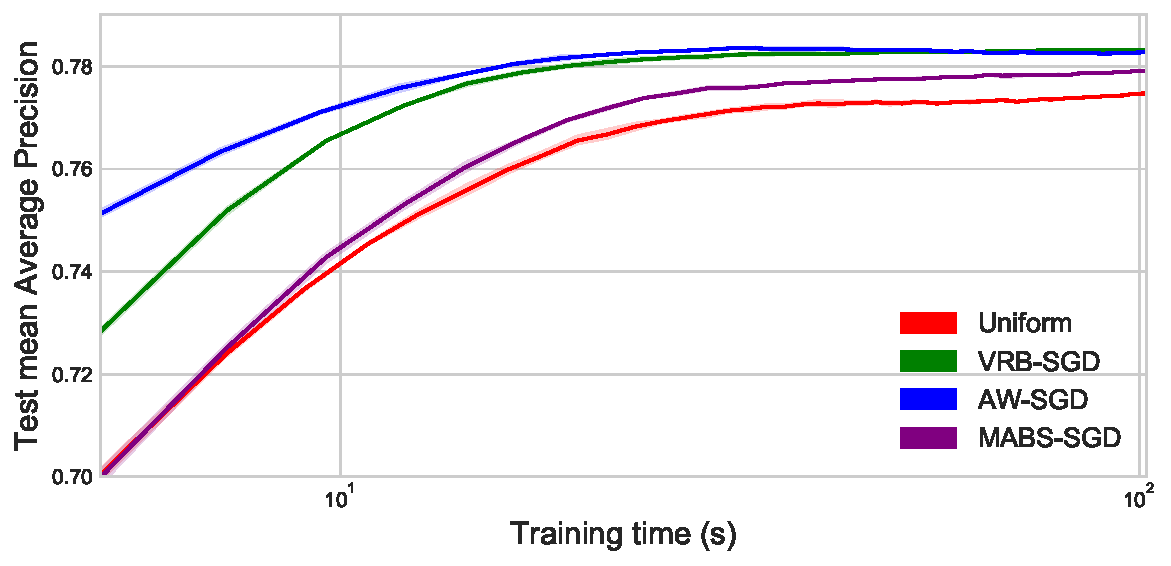
\includegraphics[width=\linewidth]{figures/voc-result.pdf}
      \caption{Mean Average Precision scores achieved on the test part of VOC 2007.}
      \label{fig:exp1}
\end{minipage}%
\quad
\begin{minipage}{.48\textwidth}
  \centering
  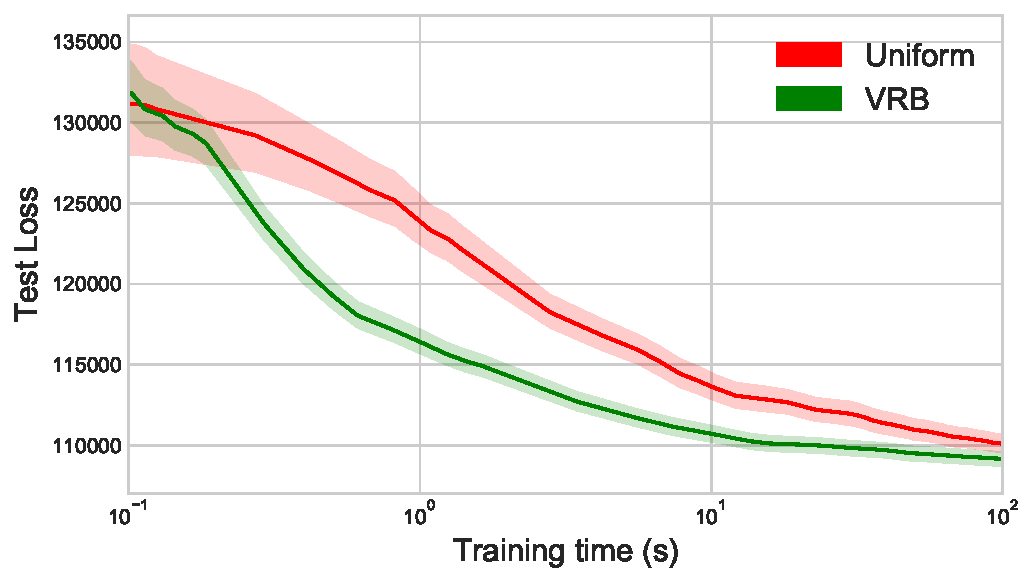
\includegraphics[width=.88\linewidth]{figures/kmeans-csn.pdf}
      \caption{$k$-Means test loss evolution on the CSN dataset.}
      \label{fig:exp2}
\label{fig:exp}
\end{minipage}%
\end{figure}
